%MARCOS RIAL DOCAMPO
%Parte del documento principal TFG

%%%%%%%%%%%%%%%%
%% RESULTADOS %%
%%%%%%%%%%%%%%%%


\chapter{Resultados}
\label{cap:resultados}

\section{Análisis de separabilidad}
\subsection{Análisis visual}
Una vez introducidos los datos en R se obtienen las gráficas mostradas en la figura \ref{fig:ral}, donde se expresan con las letras C, B, G, R e IRC la nomenclatura de las bandas de Landsat 8 ya expuestas en la sección de imágenes satélite del capítulo anterior.\Sep

%\begin{figure}
%	\centering
%	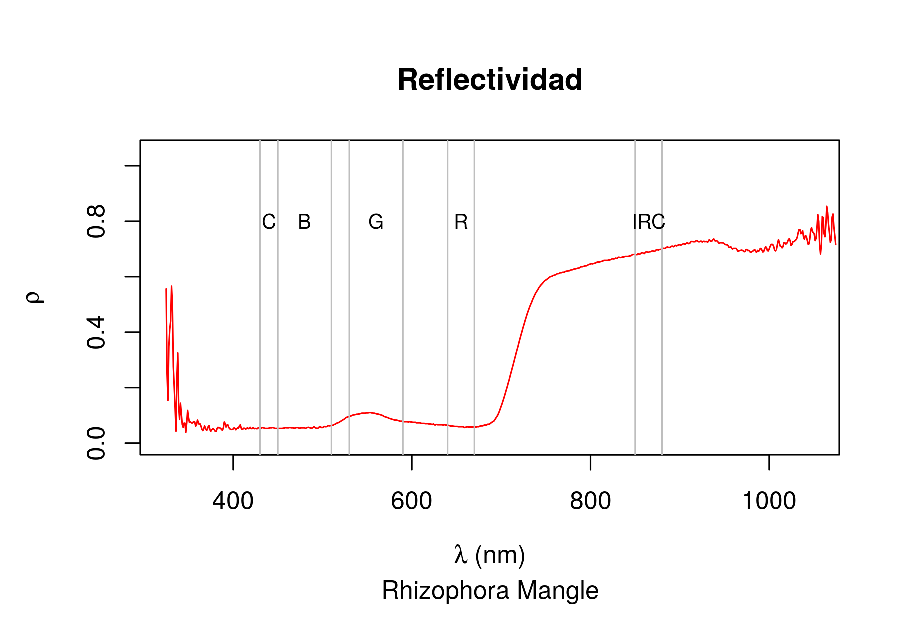
\includegraphics[width=0.8\linewidth]{./Imagenes/RM.eps}
%	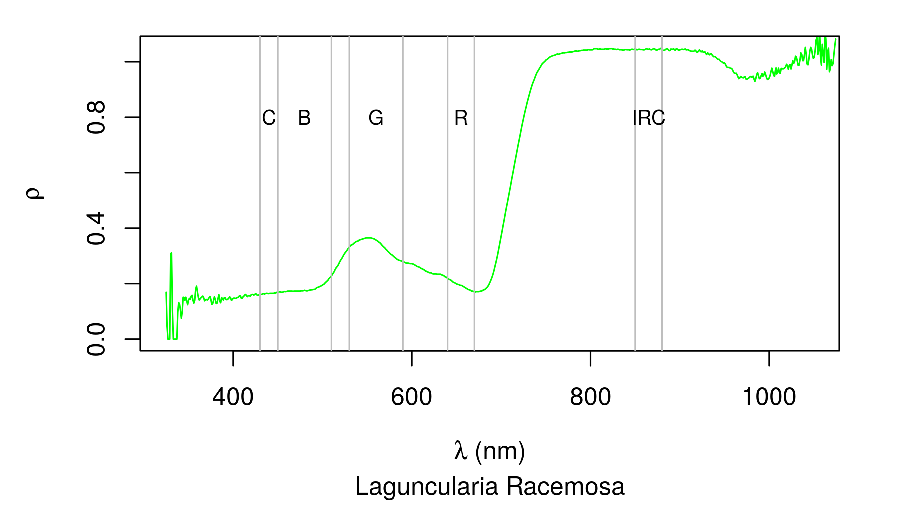
\includegraphics[width=0.8\linewidth]{./Imagenes/LR.eps}
%	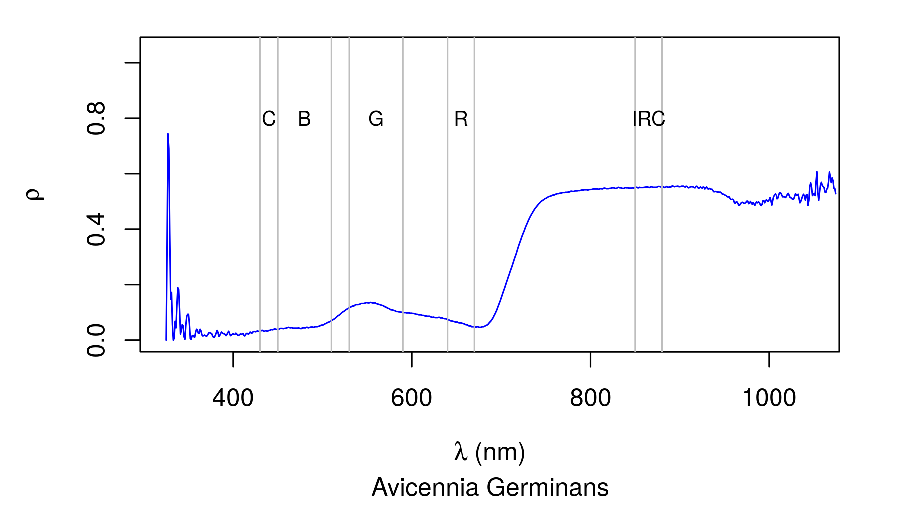
\includegraphics[width=0.8\linewidth]{./Imagenes/AG.eps}
%	\captionsetup{font={footnotesize,it}}
%	\caption[Firmas espectrales]{Gráficas de las firmas espectrales de las especies de mangle estudiadas. Fuente: Elaboración propia.}
%	\label{fig:firmas_espectrales}
%\end{figure}

\begin{figure}
	\centering
	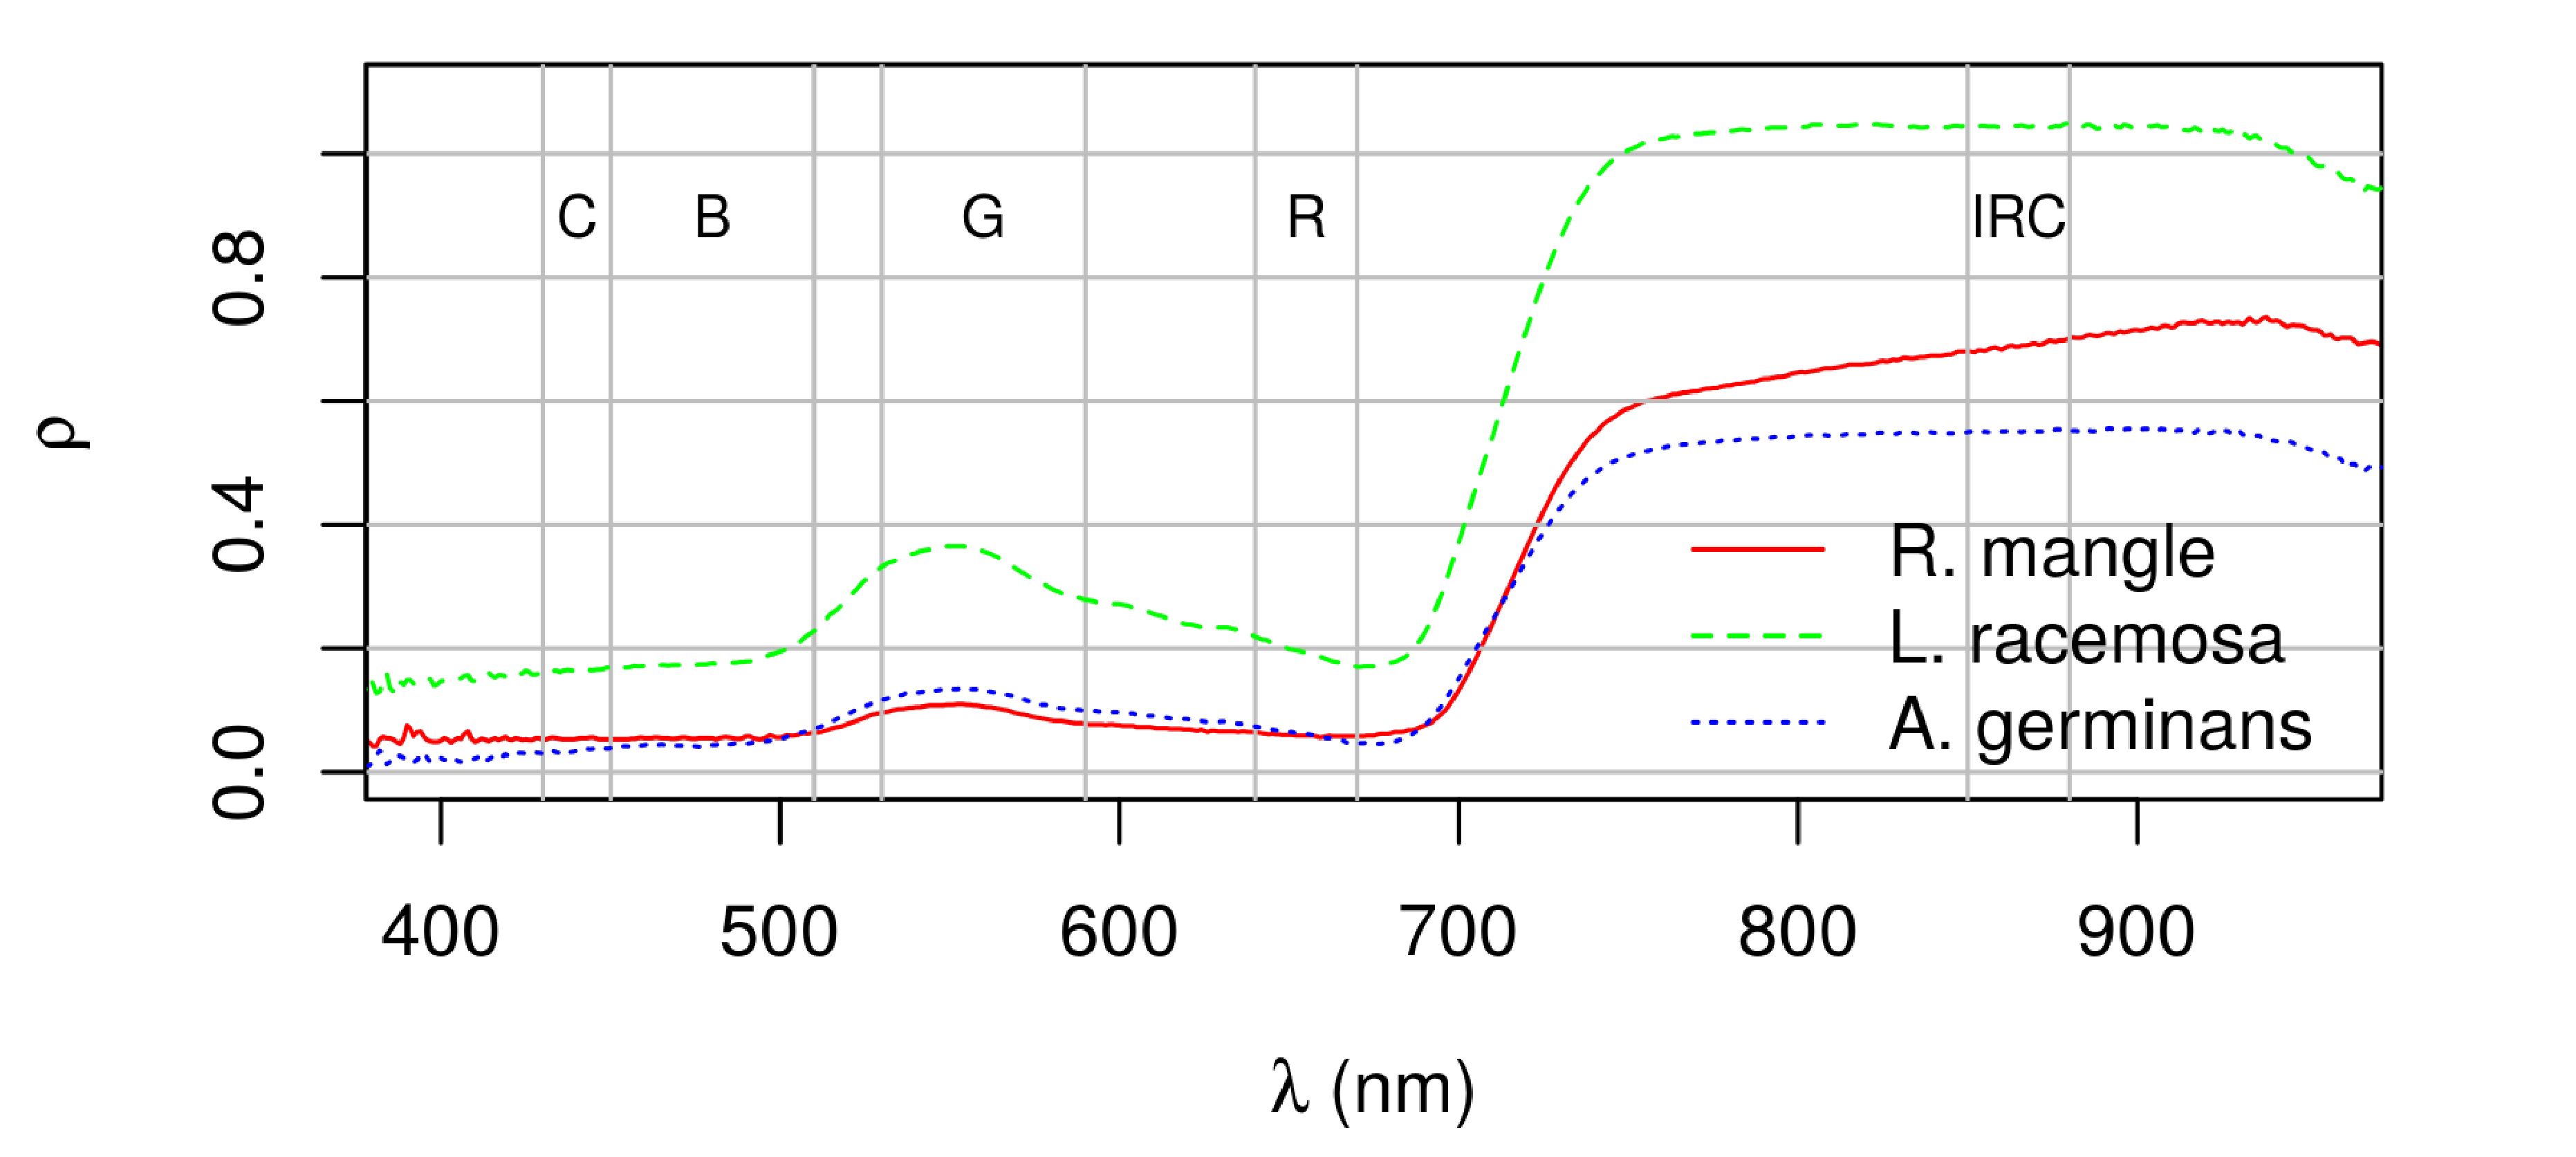
\includegraphics[width=0.8\linewidth]{./Imagenes/ral2.eps}
	\captionsetup{font={footnotesize,it}}
	\caption[Firmas espectrales de las tres especies]{Gráfica conjunta de las tres firmas espectrales. Elaboración propia.}
	\label{fig:ral}
\end{figure}

Como se aprecia, los datos presentan unas alteraciones al inicio y al final que son propias del radiómetro de campo. Se procedió a desechar estos datos haciendo un corte de colas entre los valores 420 nm y 900 nm de longitud de onda para preservar lo máximo posible la integridad de los datos y que no afectaran a los análisis de separabilidad. El número de observaciones se reduciría a 481 por las 751 originales. Las gráficas resultantes son las mostradas en las figuras \ref{fig:firmas_espectrales_corte} y \ref{fig:ral_corte}.\Sep

\begin{figure}
	\centering
	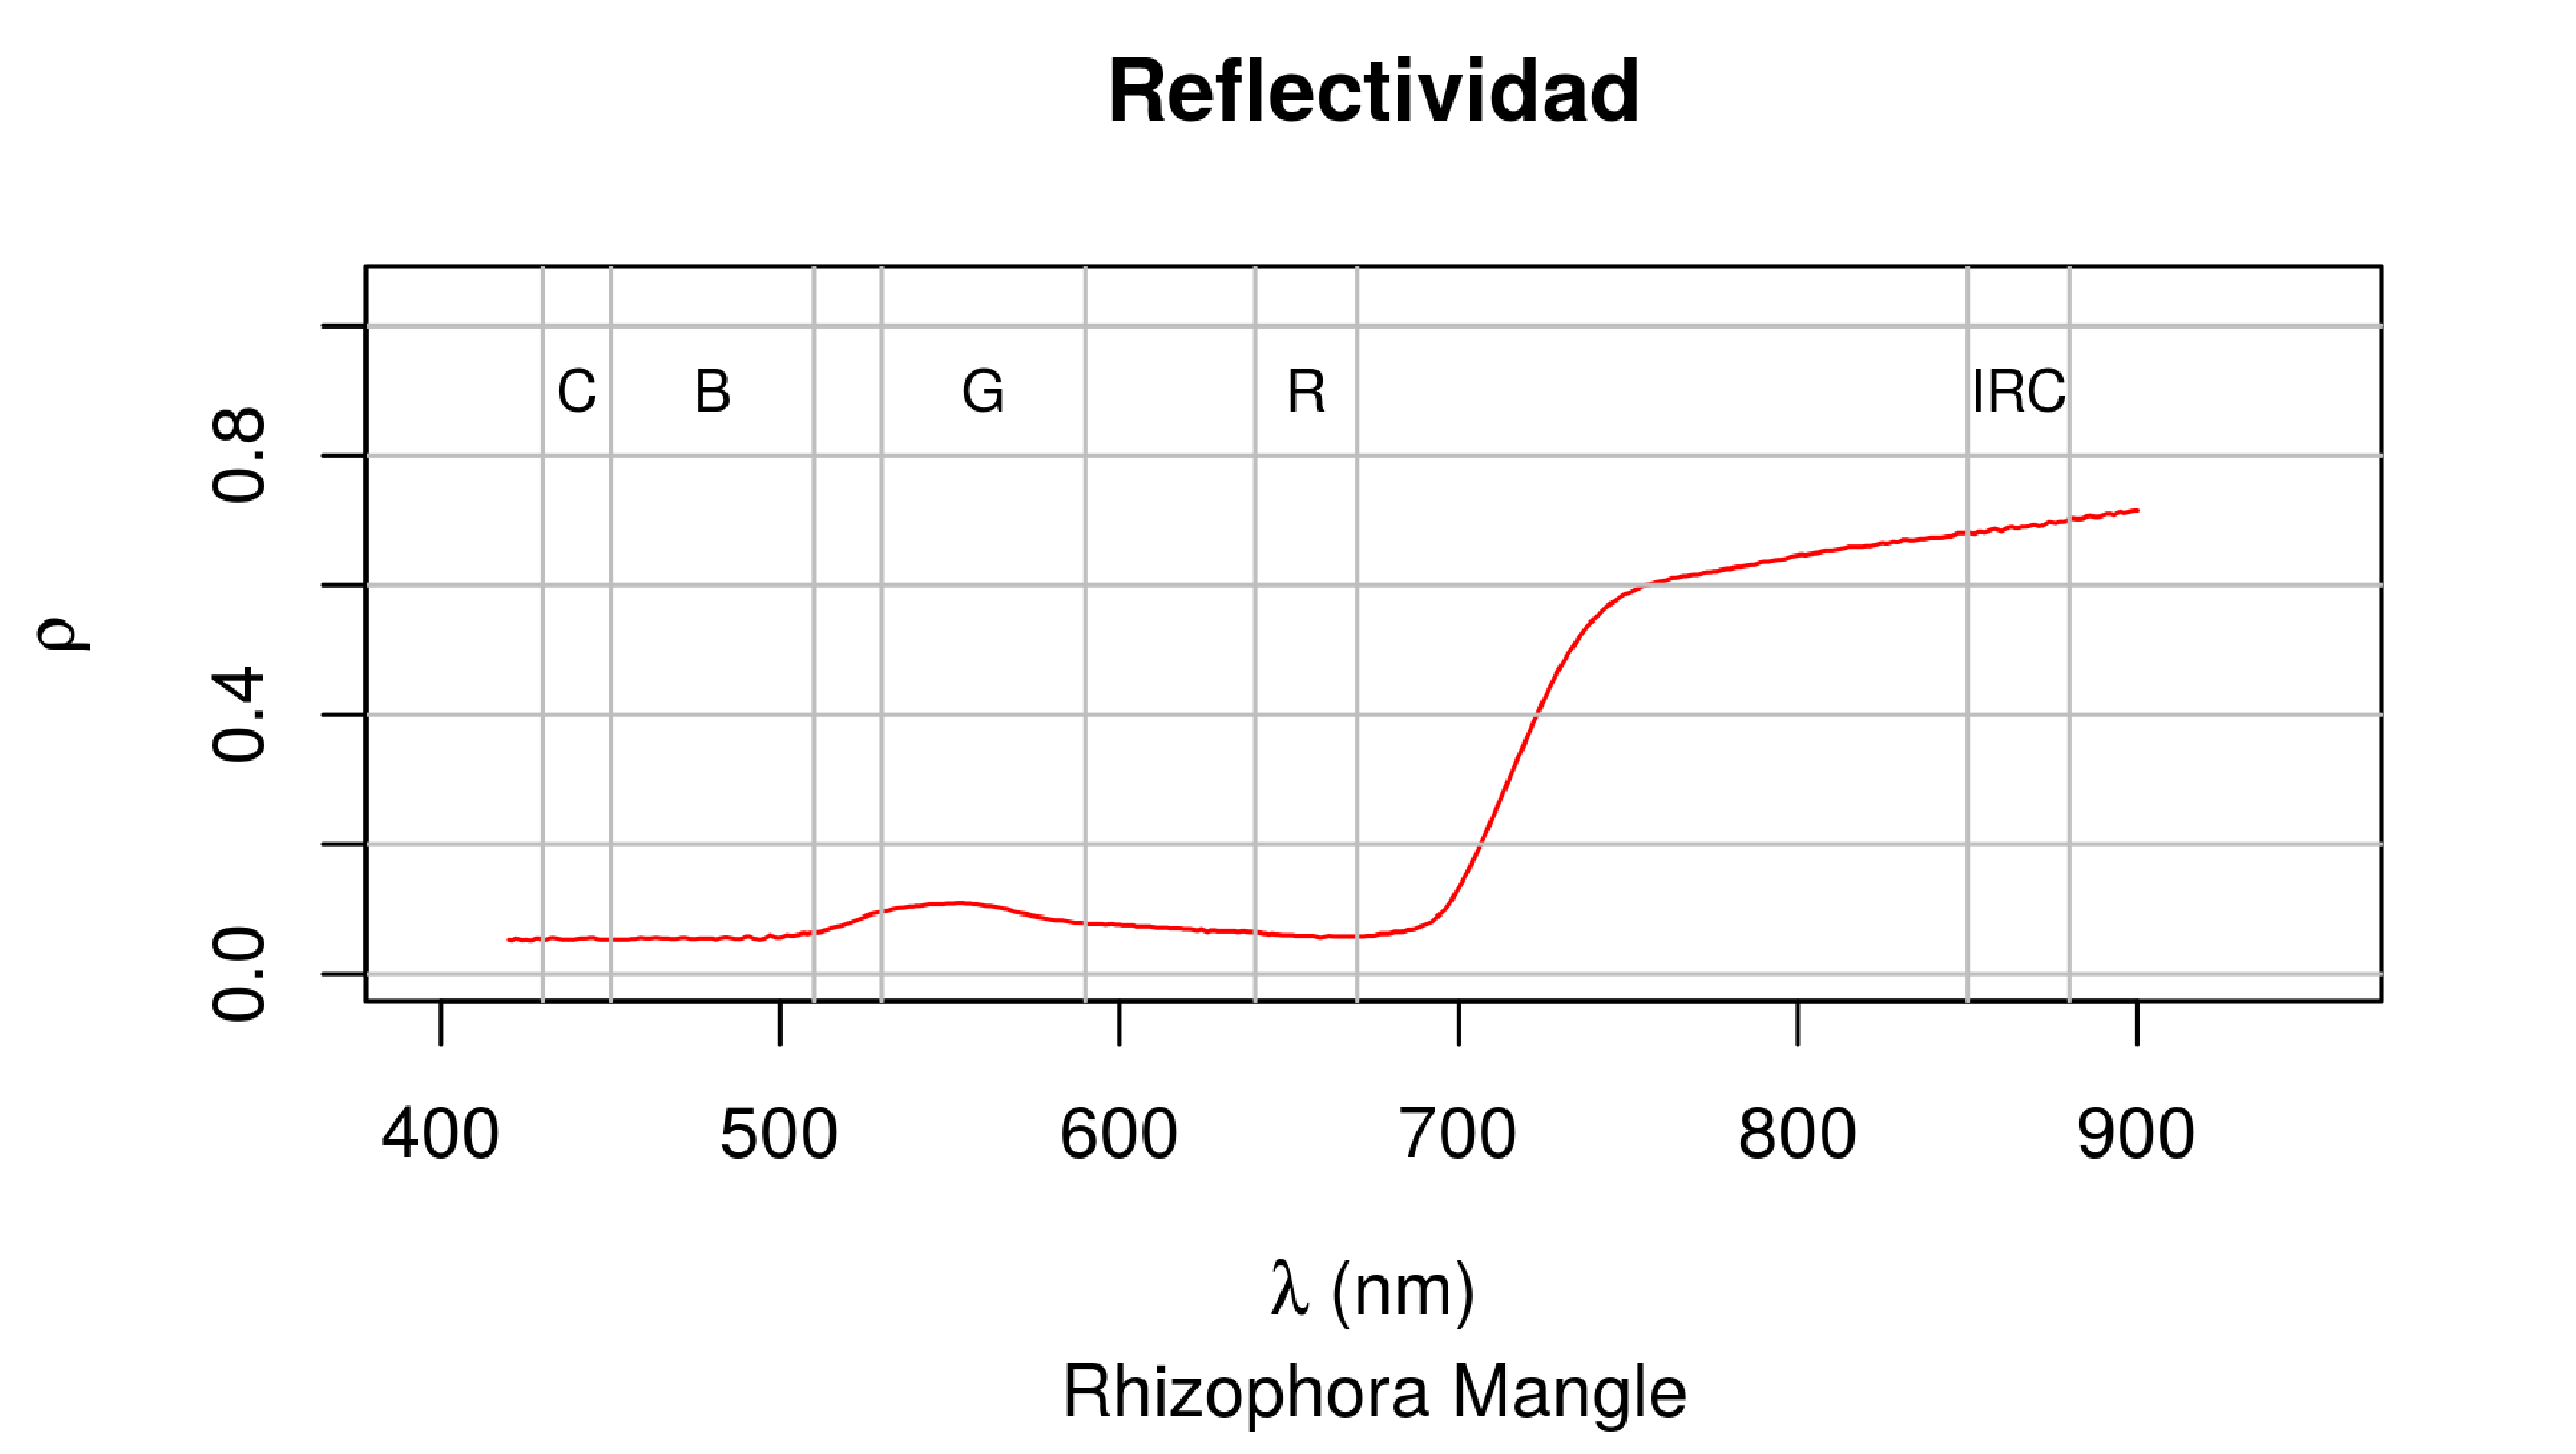
\includegraphics[width=0.8\linewidth]{./Imagenes/RMcorte.eps}
	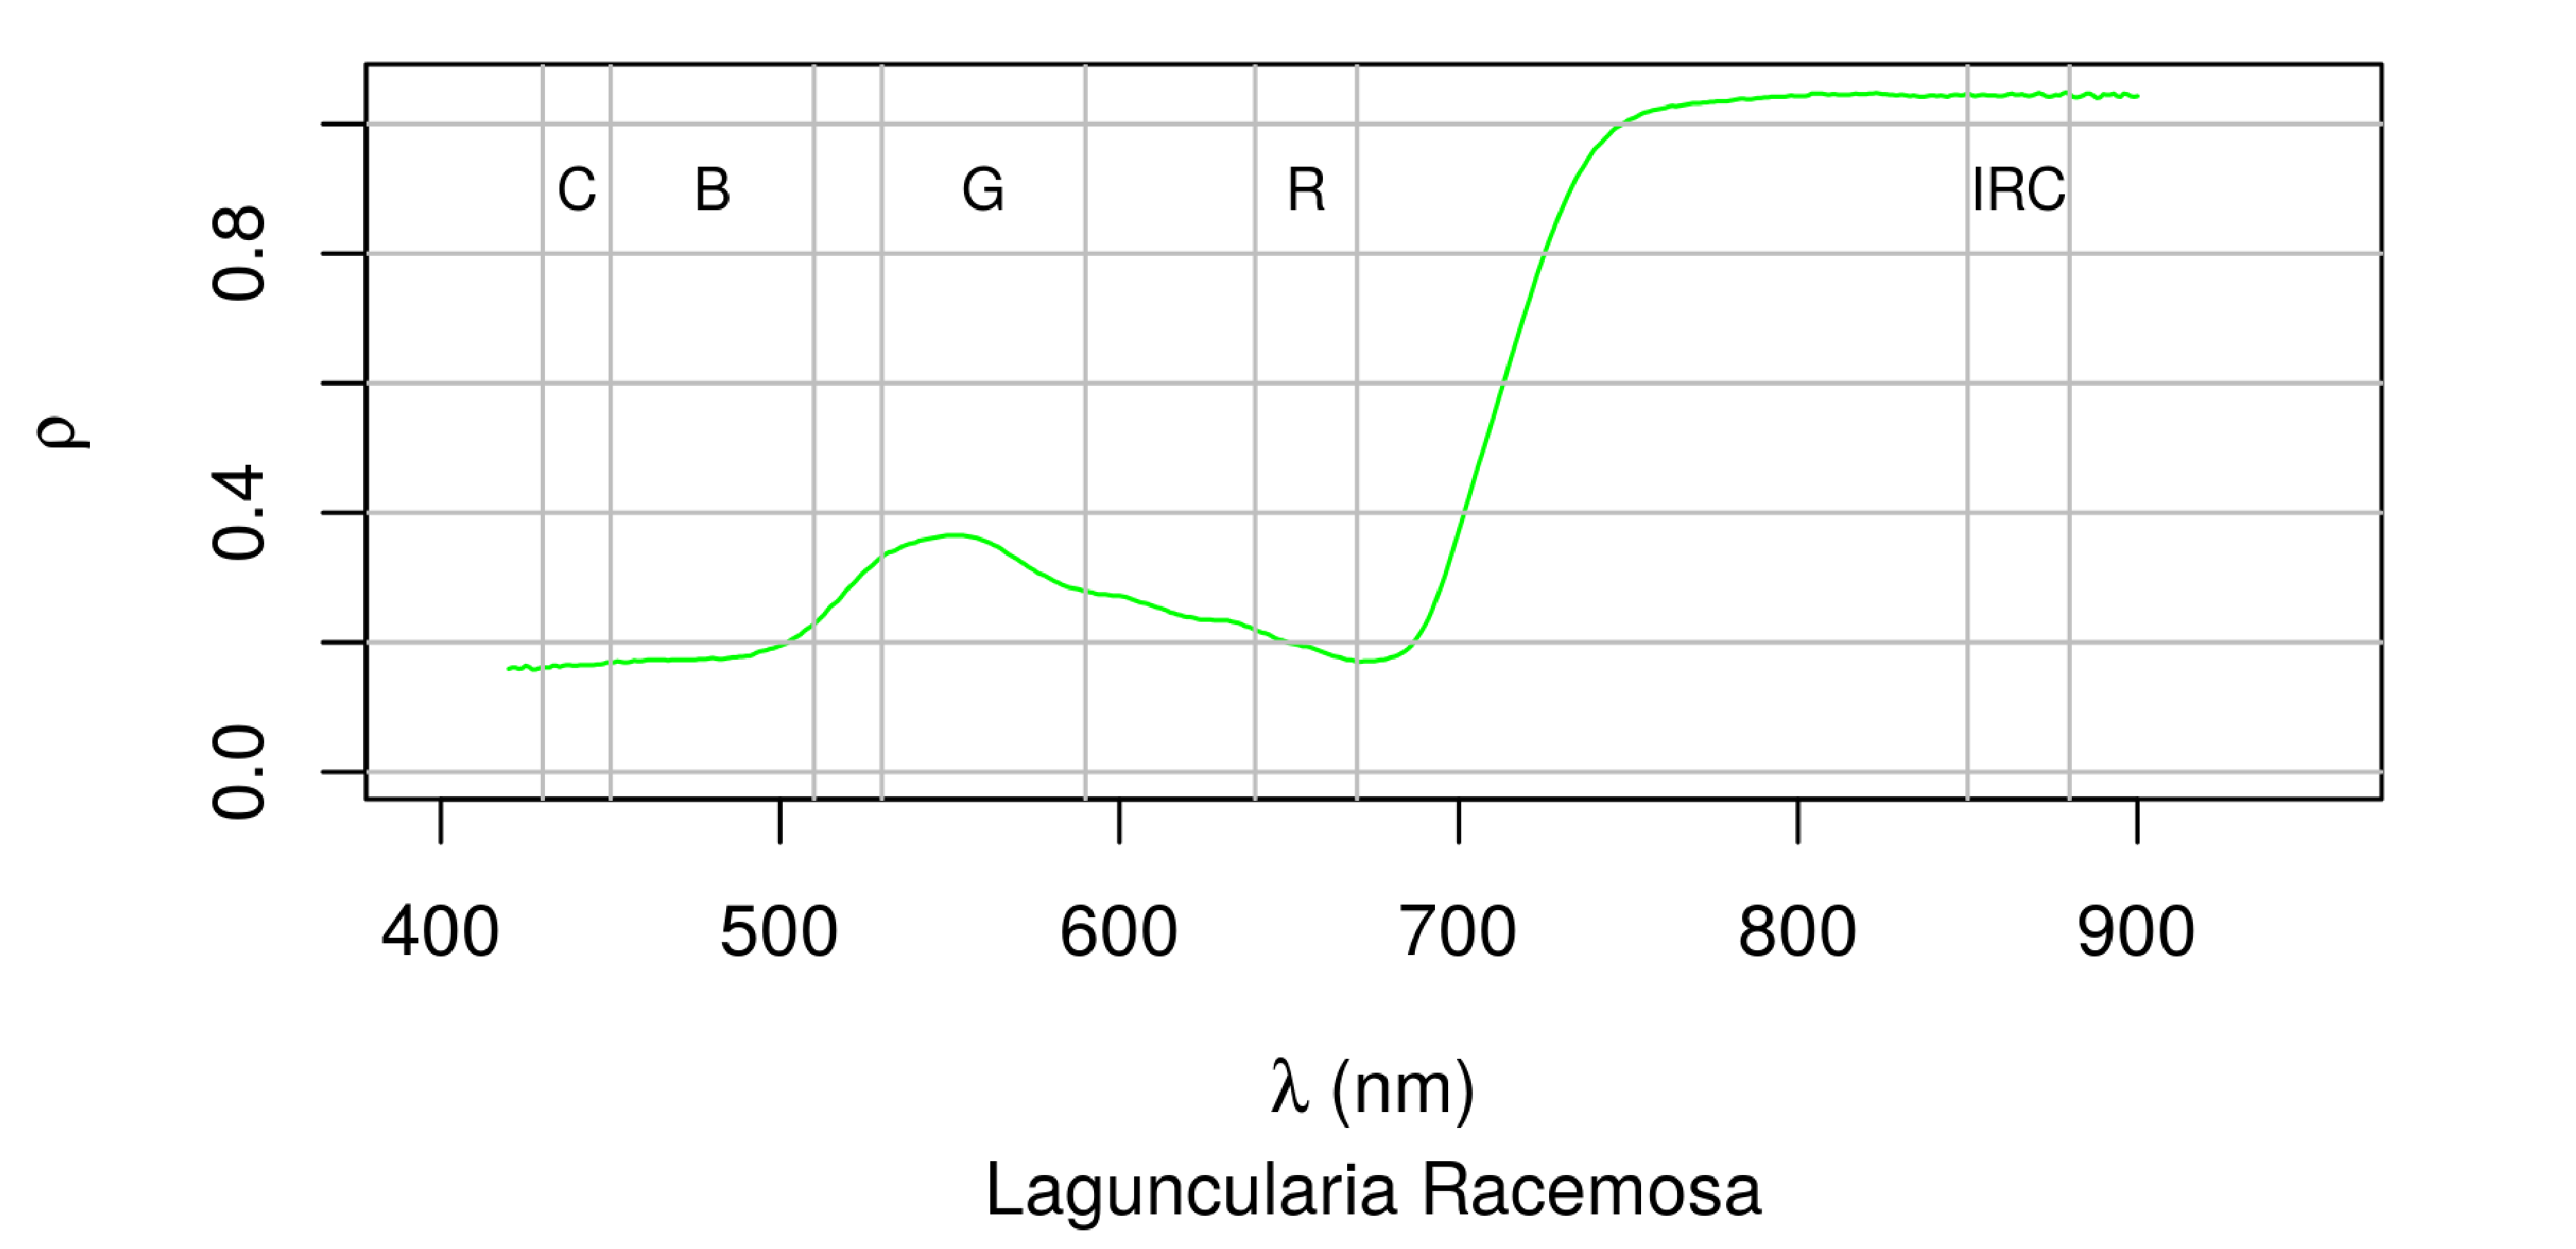
\includegraphics[width=0.8\linewidth]{./Imagenes/LRcorte.eps}
	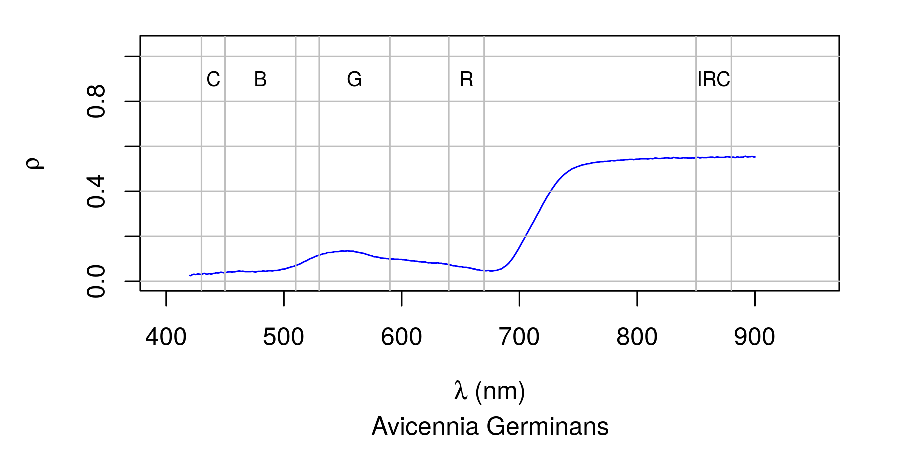
\includegraphics[width=0.8\linewidth]{./Imagenes/AGcorte.eps}
	\captionsetup{font={footnotesize,it}}
	\caption[Firmas espectrales cortadas]{Gráficas de las firmas espectrales de las especies de mangle estudiadas una vez realizado el corte de los datos. Elaboración propia.}
	\label{fig:firmas_espectrales_corte}
\end{figure}

\begin{figure}
	\centering
	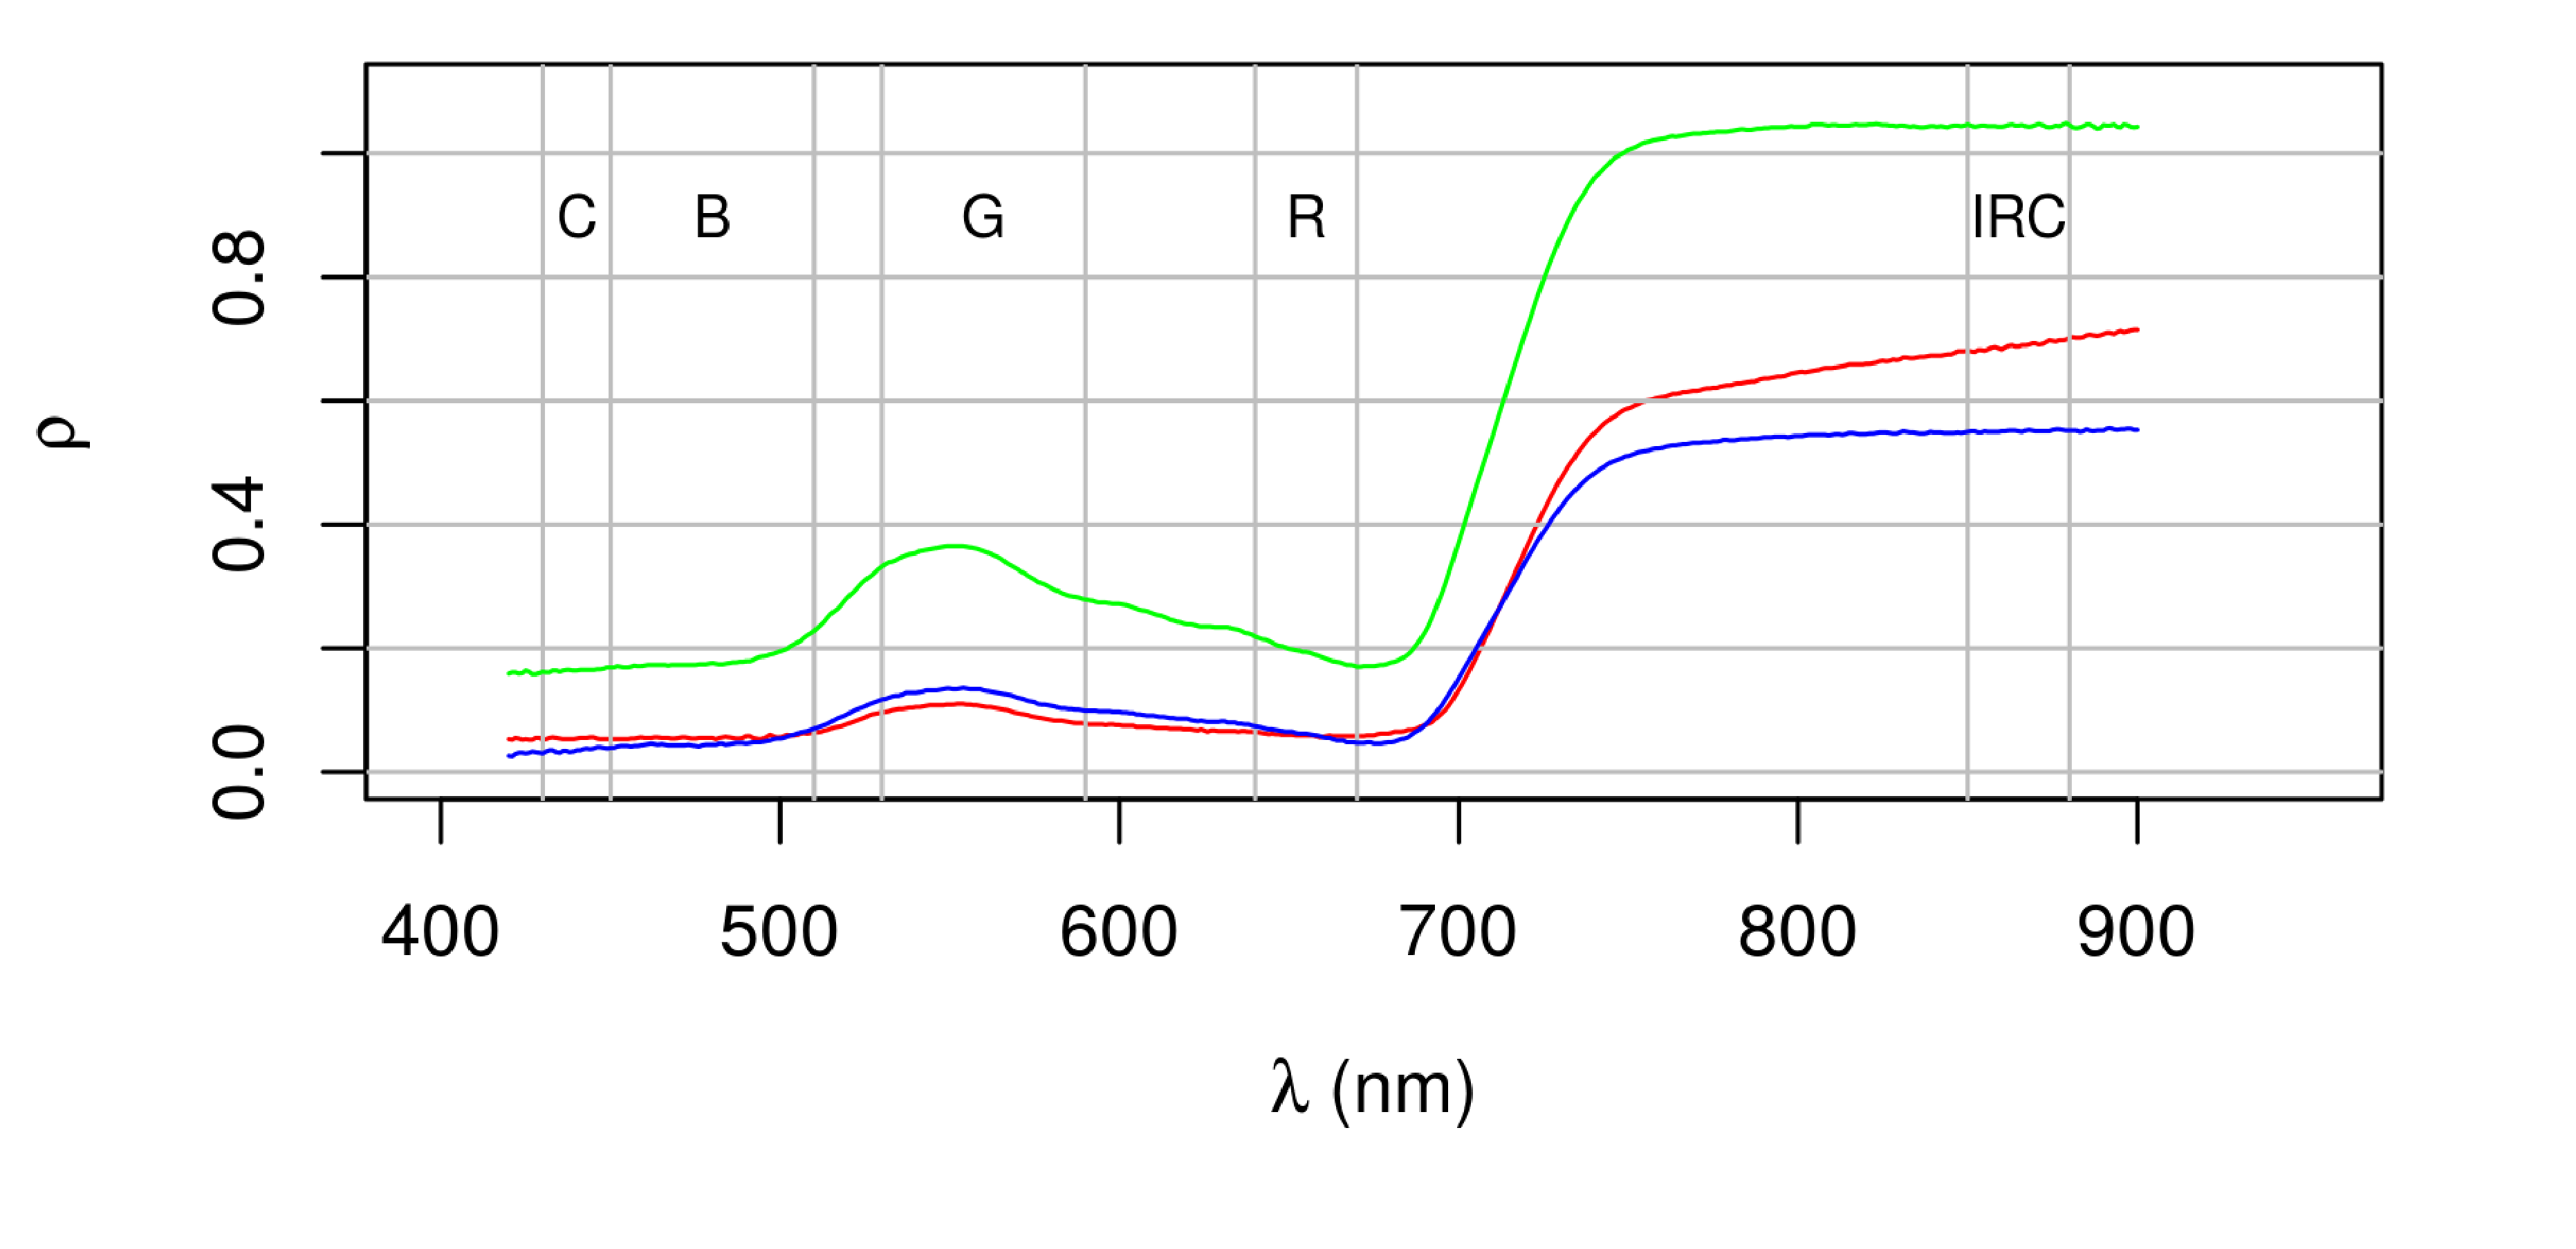
\includegraphics[width=0.8\linewidth]{./Imagenes/ralcorte.eps}
	\captionsetup{font={footnotesize,it}}
	\caption[Firmas espectrales cortadas de las tres especies]{Gráfica conjunta de las tres firmas espectrales una vez realizado el corte de los datos. Elaboración propia.}
	\label{fig:ral_corte}
\end{figure}

Las tres especies tienen un máximo local en la banda correspondiente al verde (G), típica de las especies vegetales, así como otro máximo de mayor valor, correspondientes al intervalo de longitud de onda ($\lambda$) en el que está incluida la banda del \ac{IRC}. Este último máximo también es característico de la vegetación e indicaría su grado de salud.\Sep

Por lo tanto el primer vistazo a las gráficas es el esperado, siendo lo más preocupante el aparente parecido entre las especies R. mangle y A. germinans, que solo se diferencian en los valores del rango del \ac{IRC}.\Sep

En el cuadro siguiente (\ref{tab:valores_medios}) se pueden apreciar los valores medios de cada especie para cada banda de Landsat 8.

\begin{table}[ht]
	\centering
	\begin{tabular}{@{}cccccc@{}}
	\toprule[0.4mm]
	Especie & Banda 1 (C) & Banda 2 (B) & Banda 3 (G) & Banda 4 (R) & Banda 5 (IRC) \\
	\midrule
	\textit{R. mangle}	& 0.0540 & 0.0561 & 0.0980 & 0.0595 & 0.6895 \\
	\textit{L. racemosa} & 0.1647 & 0.1821 & 0.3345 & 0.1930 & 1.0445 \\
	\textit{A. germinans} & 0.0355 & 0.0479 & 0.1218 & 0.0604 & 0.5513 \\
	\bottomrule[0.4mm]
	\end{tabular}
	\captionsetup{font={footnotesize,it}}
	\caption[Valores medios en las bandas Landsat]{Valores medios ara cada banda Landsat. Elaboración propia.}
	\label{tab:valores_medios}
\end{table}

\subsection{Índice de Acuerdo Espectral}
Una vez aplicando el script con la función de \ac{IAE} creado en R (figura \ref{fig:IAE}) ya se aprecia que el resultado no es muy bueno aunque esperado, siendo las diferencias casi inapreciables como se ve en la tabla \ref{tab:Valores_IAE}.\Sep

\begin{table}[ht]
	\centering
	\begin{tabular}{@{}cccc@{}}
	\toprule
	& \textit{R. mangle} & \textit{L. racemosa} & \textit{A. germinans} \\
	\textit{R. mangle} & --- & 0.0083 & 0.0062 \\
	\textit{L. racemosa} & 0.0083 & --- & 0.0021 \\
	\textit{A. germinans} & 0.0062 & 0.0021 & --- \\
	\bottomrule[0.4mm]
	\end{tabular}
	\captionsetup{font={footnotesize,it}}
	\caption[Valores de IAE]{Valores de \ac{IAE} para cada par de especies de mangle. Elaboración propia.}
	\label{tab:Valores_IAE}
\end{table}

Las diferencias en este método son bajas debido a que se trata de tres especies que, aunque no sean de la misma familia, si son vegetales y coexisten formando asociación en el mismo ecosistema. De haber estudiado la diferencia entre especie vegetal, suelo y agua por ejemplo, las diferencias habrían sido más notables debido a la diferencia de valor medio de la respuesta espectral. En este caso, el valor medio de las tres especies sería el mostrado en el cuadro \ref{tab:mediaIAE}.\Sep

\begin{table}
	\centering
	\begin{tabular}{@{}ccc@{}}
	\toprule[0.4mm]
	Especie & $\rho$ media & Corte en $\lambda$ (nm)\\
	\midrule
	\textit{R. mangle} & 0.2897692 & 714	\\
	\textit{L. racemosa} & 0.5424927 & 710\\
	\textit{A. germinans} & 0.2530166 & 711\\
	\bottomrule
	\end{tabular}
	\captionsetup{font={footnotesize,it}}
	\caption[Valores medios de la respuesta espectral]{Valor medio de la respuesta espectral para cada especie. Elaboración propia.}
	\label{tab:mediaIAE}
\end{table}

El corte en $\lambda$ que se menciona en el cuadro \ref{tab:mediaIAE} se refiere al valor de longitud de onda a partir del cual la reflectancia es mayor a la media y por tanto se provoca una cambio en el valor binario de 0 a 1 donde, de tener un mayor rango de longitud de onda observada habría más de un cambio. Se observan unos valores similares de $\lambda$ para las tres especies, pero donde sí se notan diferencias son en el valor medio de la reflectancia, siendo el de la \textit{L. racemosa} notablemente superior al de las otras dos especies.

\begin{comment}
\begin{figure}
	\centering
	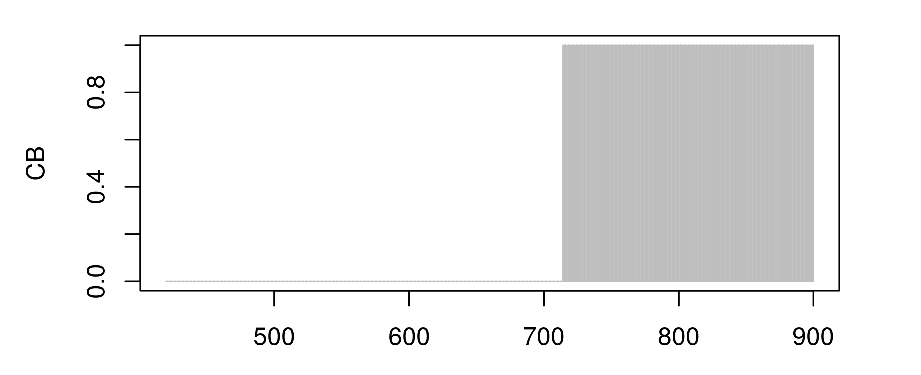
\includegraphics[width=0.8\linewidth]{./Imagenes/IAE_RM.eps}
	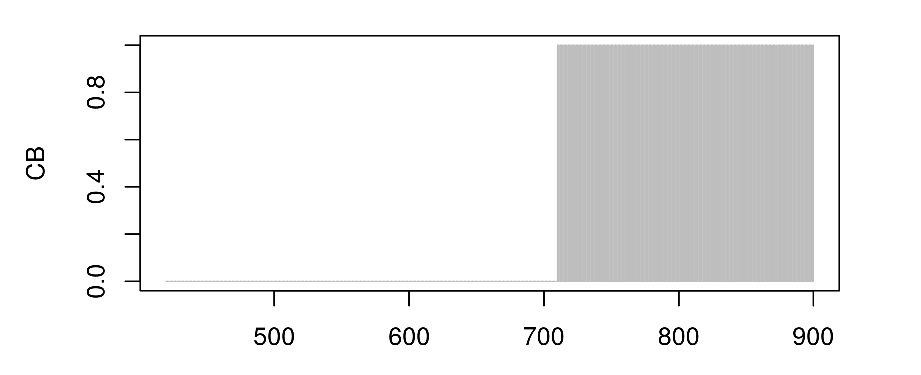
\includegraphics[width=0.8\linewidth]{./Imagenes/IAE_LR.eps}
	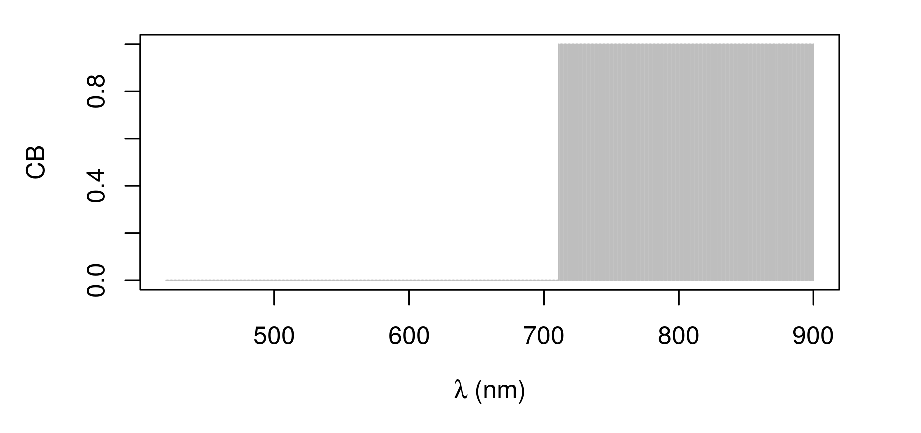
\includegraphics[width=0.8\linewidth]{./Imagenes/IAE_AG.eps}
	\captionsetup{font={footnotesize,it}}
	\caption[Gráficas de combinación binaria]{Gráficas de combinación binaria de las tres especies de mangle, por orden \textit{Rhizophora mangle}, \textit{Laguncularia racemosa} y \textit{Avicennia germinans}. Elaboración propia.}
	\label{fig:CB}
\end{figure}
\end{comment}

\subsection{\textit{Continuum Removal}}
En la gráfica de la figura \ref{fig:GraficaCR} se pueden observar las diferencias entre las tres especies que nos indica este tipo de análisis. Son tres los aspectos de esta gráfica a analizar: la profundidad y anchura de las partes convexas y la posición de los puntos mínimos. En gris la gráfica de reflectividad de cada especie.\Sep

\begin{figure}
	\centering
	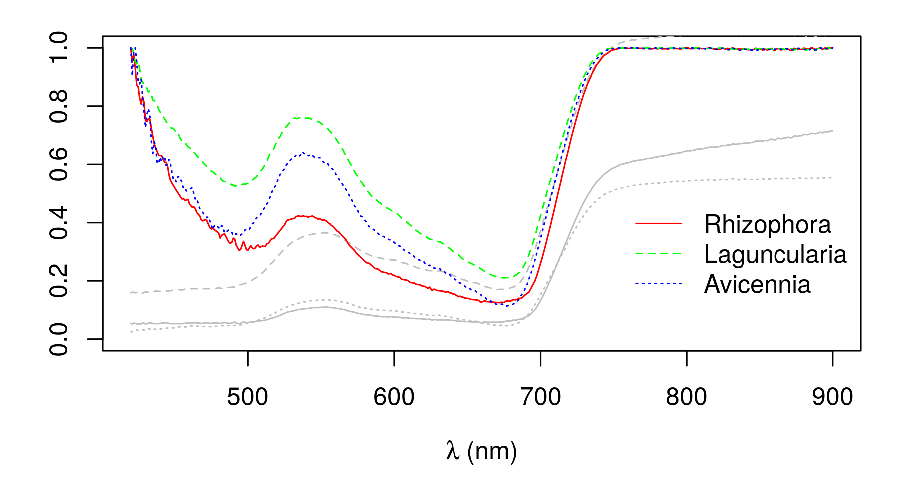
\includegraphics[width=0.8\linewidth]{./Imagenes/ContinuumR2.eps}
	\captionsetup{font={footnotesize,it}}
	\caption[Gráfica de \textit{Continuum Removal}]{Gráfica de \textit{Continuum Removal} para las tres especies de mangle. Elaboración propia.}
	\label{fig:GraficaCR}
\end{figure}

En cuanto a la profundidad se observa una clara absorción en torno a los 490 nm y los 680 nm de las tres especies. En el caso de la \textit{A. germinans} esta absorción es más acusada en ambos puntos. \textit{R. mangle} y \textit{L. racemosa} muestran un comportamiento similar en la primera zona mientras que en la segunda la \textit{L. racemosa} no muestra la absorción de la \textit{R. mangle}.\Sep

En cuanto a la anchura lo más llamativo es la amplitud de los valores de la \textit{R. mangle} en torno a los valores centrales de la observación.

\subsection{Clasificación angular}
Una vez aplicado el script de R de la función de clasificación angular (figura \ref{fig:AE}), los valores son los de la siguiente tabla:

\begin{table}[ht]
	\centering	
	\begin{tabular}{@{}cccc@{}}
	\toprule[0.4mm]
	& \textit{R. mangle} & \textit{L. racemosa} & \textit{A. germinans} \\
	\textit{R. mangle} & --- & 0.1651 (10.5085) & 0.0752 (4.7874) \\
	\textit{L. racemosa} & 0.1651 (10.5085) & --- & 0.1062 (6.7584) \\
	\textit{A. germinans} & 0.0752 (4.7874) & 0.1062 (6.7584) & --- \\
	\bottomrule[0.4mm]
	\end{tabular}
	\captionsetup{font={footnotesize,it}}
	\caption[Valores de Ángulo Espectral]{Valores del Ángulo Espectral en radianes. Ángulo centesimal entre paréntesis. Elaboración propia.}	
\end{table}

Se puede observar una mayor separabilidad entre \textit{R. mangle} y \textit{L. racemosa}, siendo menor en las otras combinaciones.

\section{Combinación de bandas}
Para observar las zonas donde hay presencia de bosque de mangle basta con realizar diversas combinaciones de bandas de Landsat 8. A las figuras ya expuestas en el capítulo de materiales y métodos (figuras \ref{fig:gf432} y \ref{fig:gf543}) correspondientes al color real y a un falso color con realce del \ac{IRC} en el canal rojo. En las figuras \ref{fig:gf654} y \ref{fig:gf562} se muestran combinaciones que también buscan conseguir un realce del manglar. Por las propiedades de reflectividad de la cubierta combinando bandas del infrarrojo se obtienen buenos resultados para realizar un análisis visual.

\begin{figure}
	\centering
	\includegraphics[width=0.8\linewidth]{./Imagenes/GF654.eps}
	\captionsetup{font={footnotesize,it}}
	\caption[Composición 654]{Resultado de la imagen en una composición de realce de vegetación (6-5-4). Imagen exportada de GRASS. Elaboración propia.}
	\label{fig:gf654}
\end{figure}

\begin{figure}
	\centering
	\includegraphics[width=0.8\linewidth]{./Imagenes/GF562.eps}
	\captionsetup{font={footnotesize,it}}
	\caption[Composición 562]{Resultado de la imagen en una composición de realce de vegetación (5-6-2). Imagen exportada de GRASS. Elaboración propia.}
	\label{fig:gf562}
\end{figure}

\section{Comprobación}
Debido a que en la corrección utilizada en las imágenes \ac{PL8SR} los valores vienen presentados con un factor de escala de 0.0001 \citep{USGS2015} corresponde reescalar los valores a un intervalo 0-1 más común. Para ello se emplea la calculadora de mapas ráster de GRASS aplicando la expresión $L8GF\_SRFB1@TFG \cdot 0.0001$ para cada una de las capas del proyecto. La línea de comando utilizada es la siguiente:

\begin{figure}[ht]
	\centering
	\begin{boxedverbatim}
	r.mapcalc `L8GF_B1=L8GF_SRFB1@TFG*0.0001'
	\end{boxedverbatim}
	\captionsetup{font={footnotesize,it}}
	\caption[Reescalado de valores]{Reescalado de los valores de la imagen Landsat con r.mapcalc.}
\end{figure}

Se muestran los valores resultantes para cada punto en el cuadro \ref{tab:tabla_puntos} y su distribución en la zona de estudio en la figura \ref{fig:dist_puntos}.\Sep

\begin{table}[ht]
	\centering
	\begin{tabular}{@{}cccccccc@{}}
	\toprule[0.4mm]
	cat & x & y & B1 & B2 & B3 & B4 & B5\\
	\midrule
	1 & 413076.12 & 1485451.42 & 0.0080 & 0.0102 & 0.0249 & 0.0120 & 0.3054\\
	2 & 416539.92 & 1483130.35 & 0.0096 & 0.0113 & 0.0254 & 0.0137 & 0.2964\\
	3 & 413619.63 & 1482194.38 & 0.0090 & 0.0108 & 0.0247 & 0.0116 & 0.3311\\
	4 & 434978.06 & 1485551.73 & 0.0076 & 0.0099 & 0.0256 & 0.0124 & 0.3132\\
	5 & 435666.27 & 1481906.87 & 0.0086 & 0.0109 & 0.0254 & 0.0134 & 0.2954\\
	6 & 426223.06 & 1479693.58 & 0.0106 & 0.0131 & 0.0330 & 0.0173 & 0.2963\\
	7 & 434938.70 & 1478948.70 & 0.0119 & 0.0146 & 0.0309 & 0.0190 & 0.2612\\
	8 & 455289.36 & 1479452.68 & 0.0132 & 0.0163 & 0.0385 & 0.0268 & 0.2300\\
	9 & 447490.46 & 1478621.82 & 0.0147 & 0.0187 & 0.0413 & 0.0286 & 0.2300\\
	10 & 452584.20 & 1462969.61 & 0.0115 & 0.0143 & 0.0345 & 0.0209 & 0.2577\\
	\bottomrule[0.4mm]
	\end{tabular}
	\captionsetup{font={footnotesize,it}}
	\caption[Base de datos de puntos de comprobación]{Base de datos asociada a la capa vectorial ``puntos'' de la figura \ref{fig:dist_puntos}. Elaboración propia.}
	\label{tab:tabla_puntos}
\end{table}

\begin{figure}
	\centering
	\includegraphics[width=0.8\linewidth]{./Imagenes/puntos_comprob.eps}
	\captionsetup{font={footnotesize,it}}
	\caption[Distribución de puntos]{Distribución de puntos de comprobación en la zona de estudio. Elaboración propia.}
	\label{fig:dist_puntos}
\end{figure}

Para hacer una comprobación de los datos tomados en campo se superponen estos a una gráfica de cajas y bigotes extraída de los valores de los puntos de comprobación (figura \ref{fig:grafica_comprob}). Un gráfico de este tipo consiste en una caja rectangular donde los lados verticales (en nuestro caso) muestran el recorrido intercuartílico dividido por un segmento horizontal que es la mediana. Por lo tanto, de un solo vistazo nos aporta información sobre valor central (segunto cuartil), primer y tercer cuartil. Además nos dice cuales son los valores máximo y mínimo de la distribución, que formarían los bigotes, y detecta valores desfasados en forma de puntos fuera de la caja.\Sep

Gracias a esta representación gráfica se confirma que la magnitud de los datos tomados por el espectro-radiómetro de campo están incrementados en varias décimas en la lectura media de cada banda comparados con la información de las imágenes de Landsat 8. Pese a eso se puede observar como los datos tienen un aspecto similar.

\begin{figure}
	\centering
	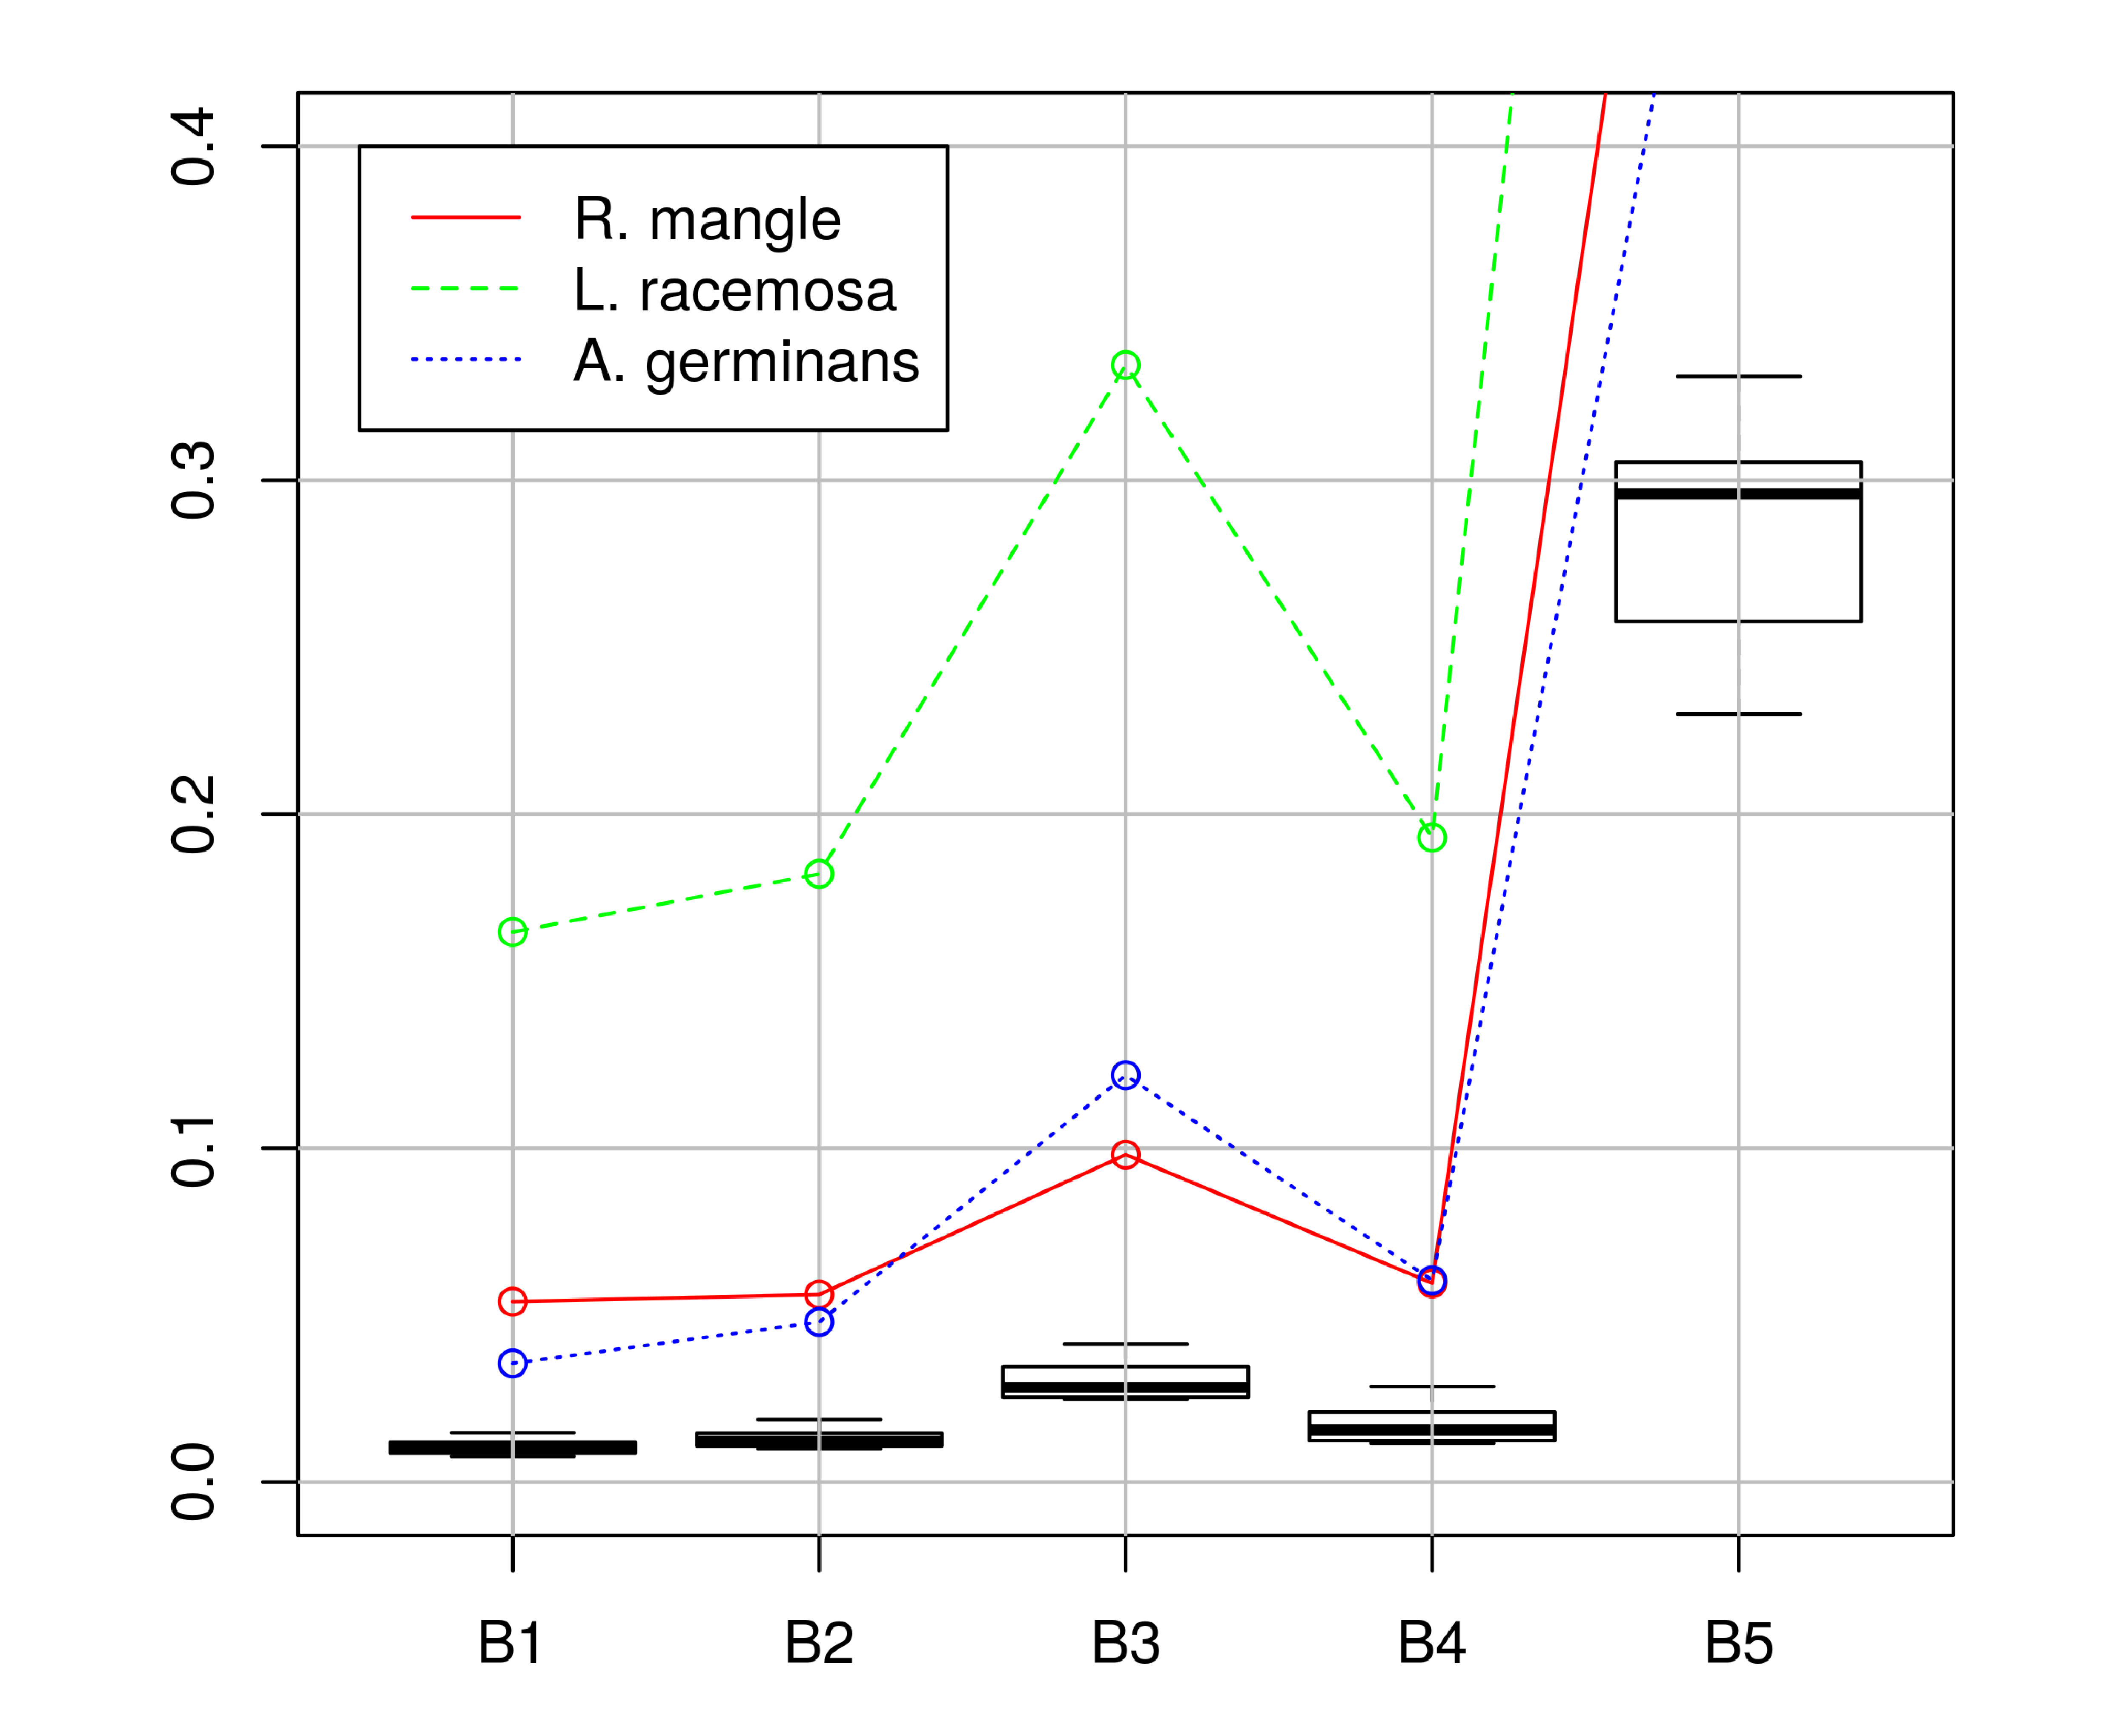
\includegraphics[width=0.8\linewidth]{./Imagenes/grafica_comprob.eps}
	\captionsetup{font={footnotesize,it}}
	\caption[Gráfico de puntos de comprobación]{Gráfico de cajas y bigotes correspondiente a los datos de los puntos de comprobación. Se superponen los datos medios de reflectividad para cada especie en cada banda. Elaboración propia.}
	\label{fig:grafica_comprob}
\end{figure}


\section{Clasificación de imágenes}
En las clasificaciones se muestra confusión de clases, mezclándose en algunos casos el mangle con otro tipo de vegetación en zonas donde, por las propias características del ecosistema, es imposible la existencia de manglar (detalle en \ref{fig:detalle_clasnosup}). A excepción de la clasificación supervisada que, a pesar de que se ve un exceso de la clase denominada ``Agua 2'' en zonas donde no hay presencia de esta, discrimina bien la cobertura de mangle de otros tipos (detalle en figura \ref{fig:detalle_classup}).\Sep

\begin{figure}
	\centering
	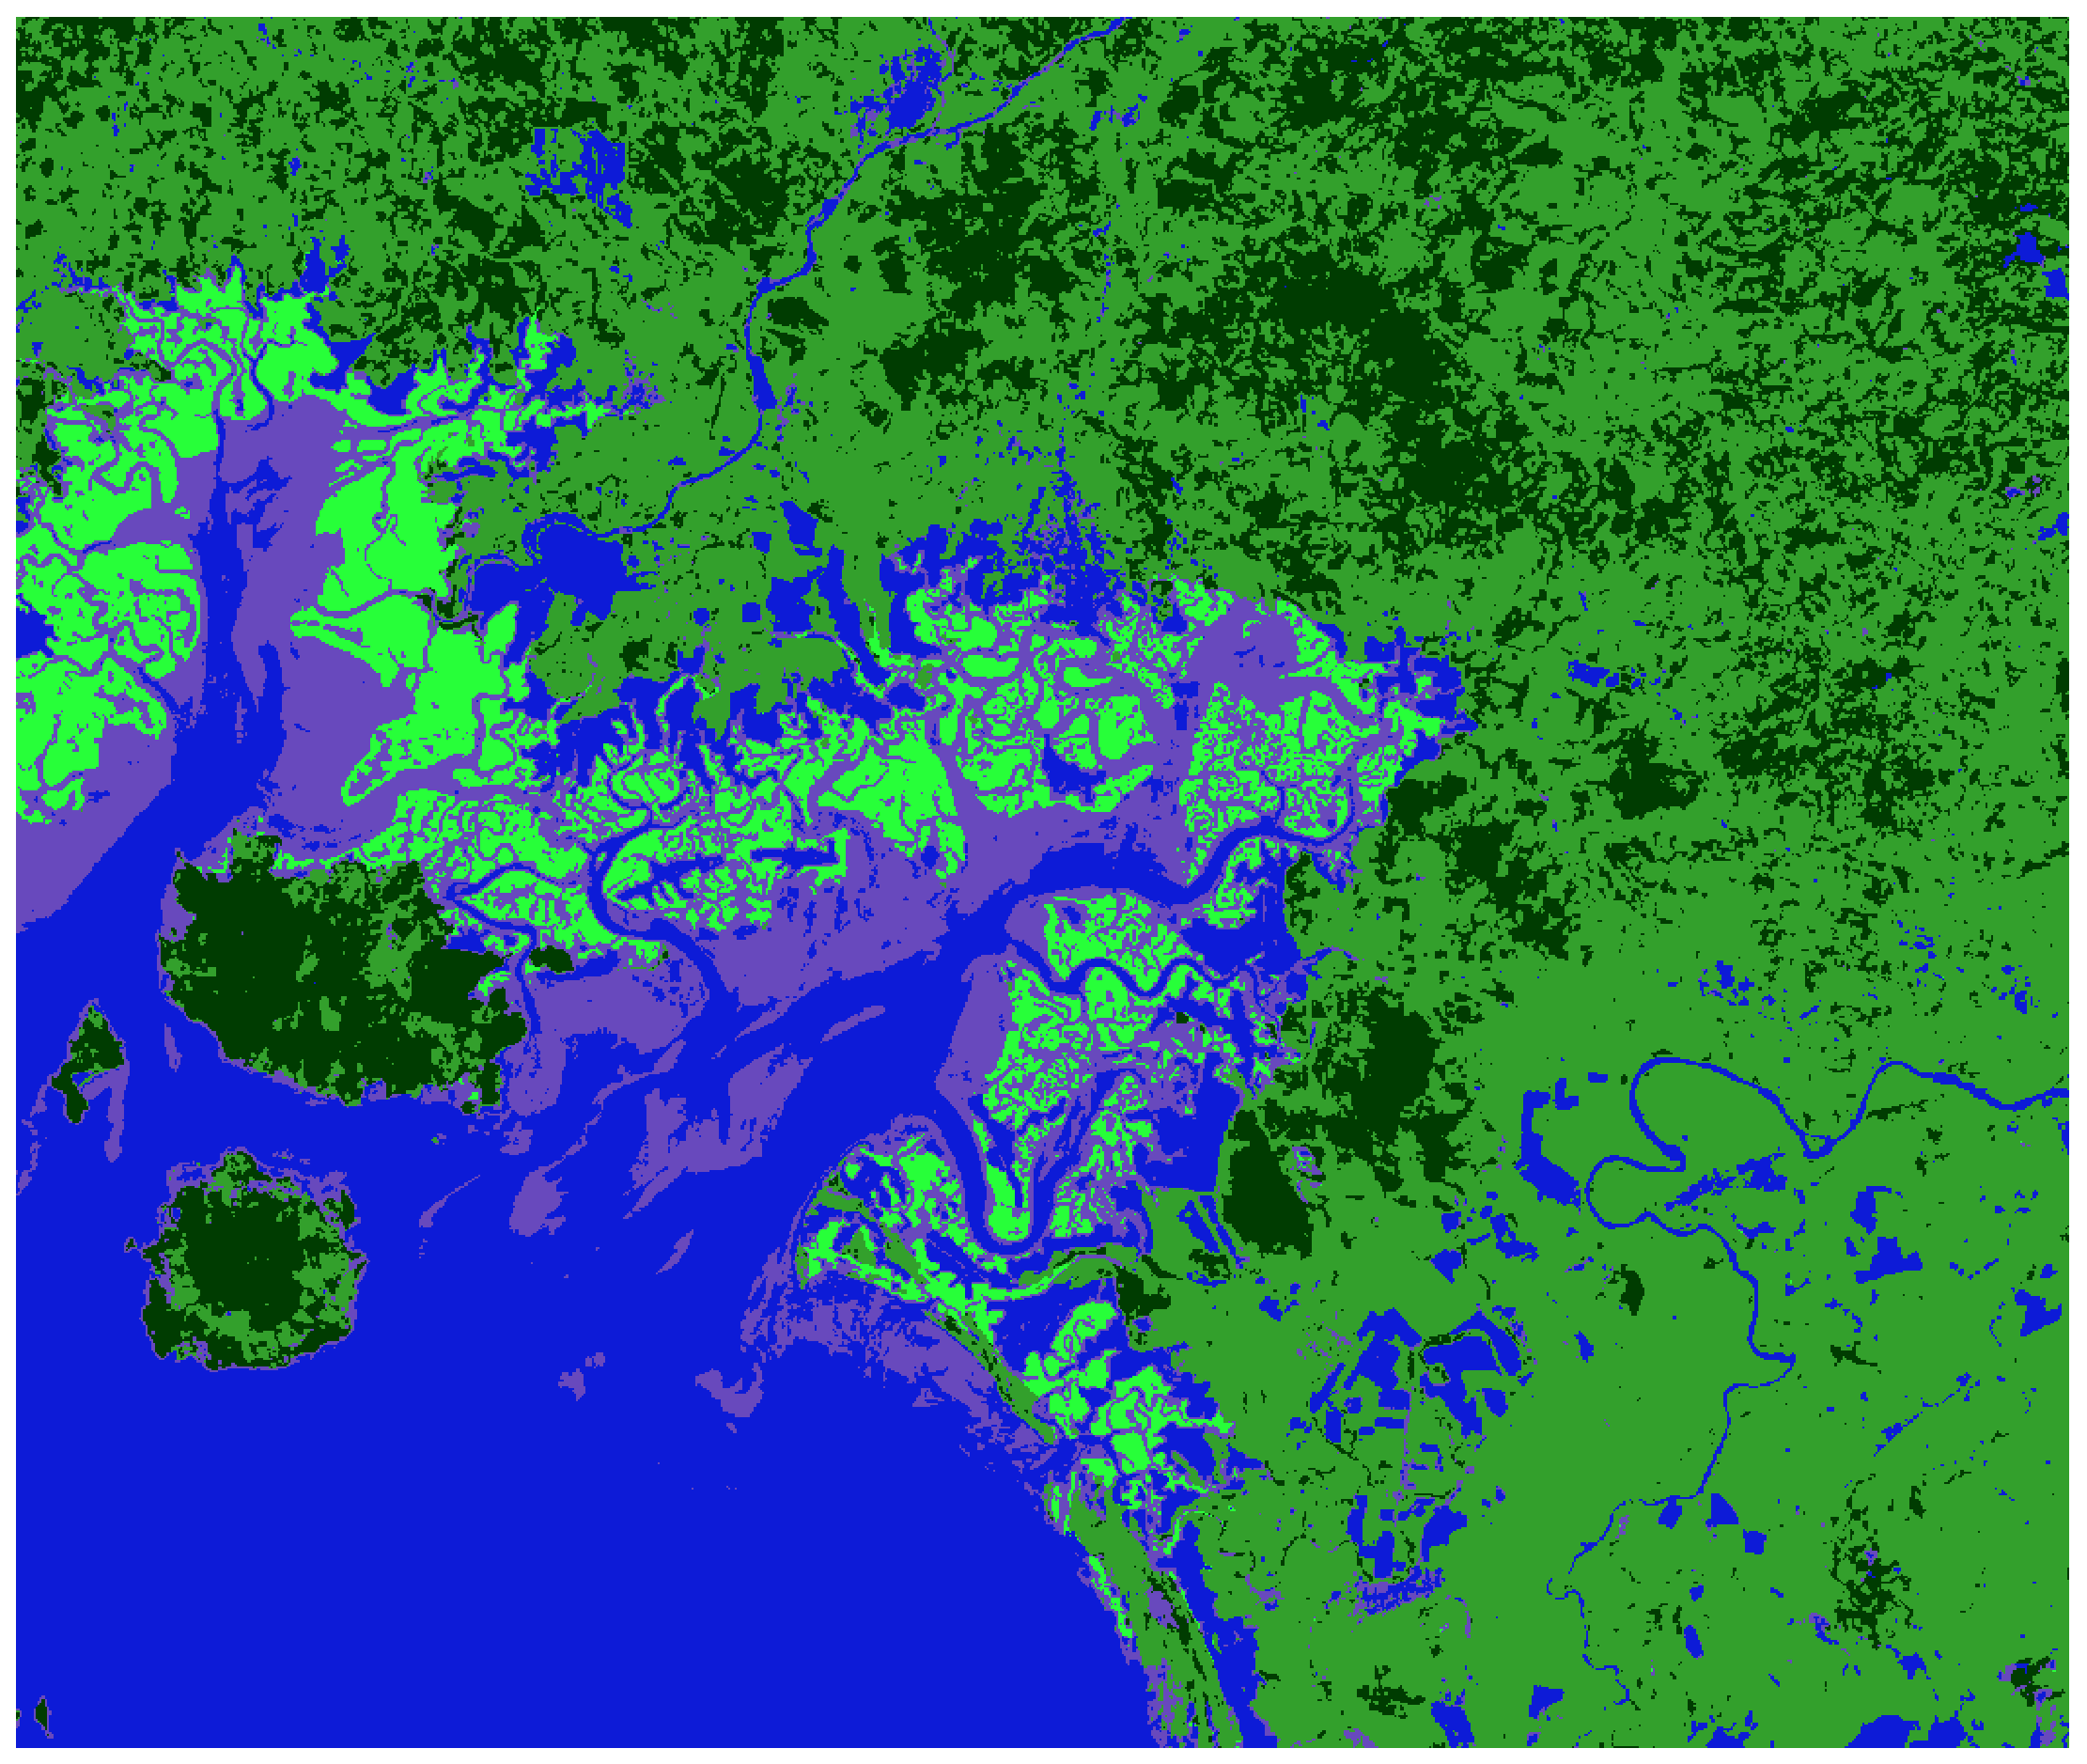
\includegraphics[width=0.8\linewidth]{./Imagenes/Detalle_classup.eps}
	\captionsetup{font={footnotesize,it}}
	\caption[Detalle clasificación supervisada]{Detalle de la clasificación supervisada. Elaboración propia.}
	\label{fig:detalle_classup}
\end{figure}

\begin{figure}
	\centering
	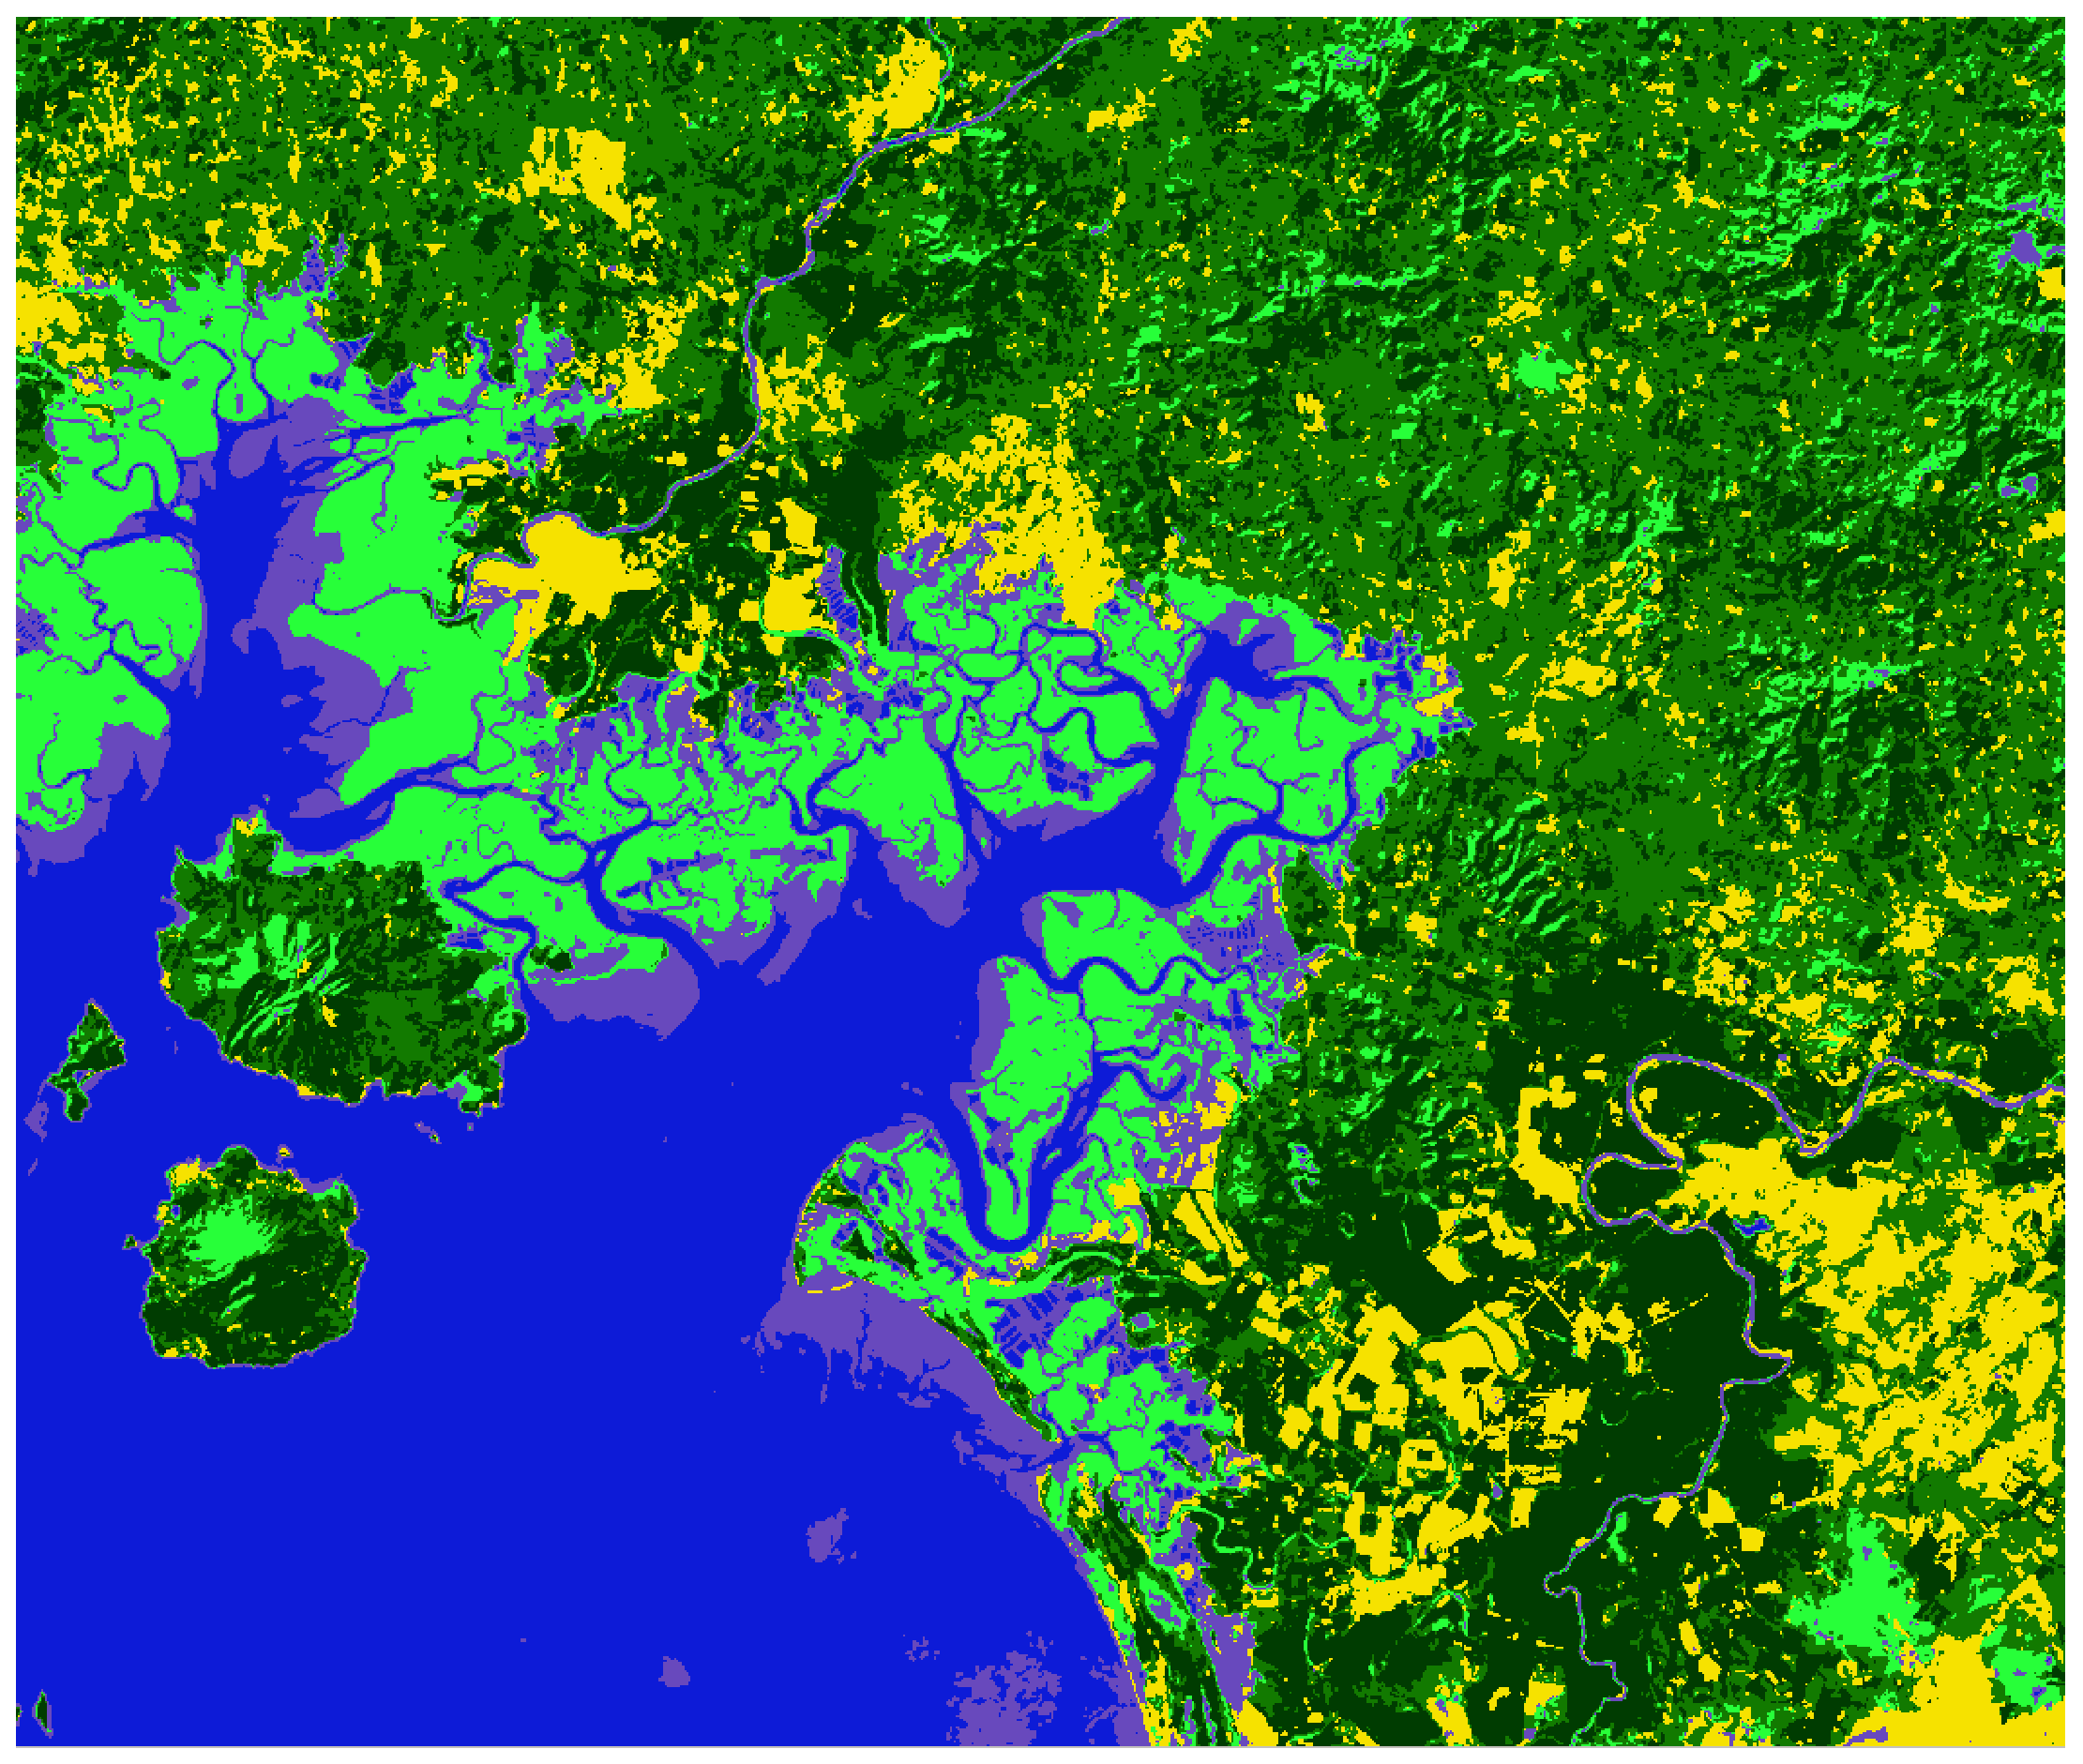
\includegraphics[width=0.8\linewidth]{./Imagenes/Detalle_clasnosup.eps}
	\captionsetup{font={footnotesize,it}}
	\caption[Detalle clasificación no supervisada]{Detalle de la clasificación no supervisada. Elaboración propia.}
	\label{fig:detalle_clasnosup}
\end{figure}

Se muestra el resultado de las clasificaciones en el anejo de mapas de este documento.

\section{Índices de vegetación}
El \ac{NDVI} nos muestra más claramente zonas de marisma o aguas turbias poco profundas que se sitúan en la línea de costa (figura \ref{fig:detalle_aguas}), justo donde hay presencia de bosque de mangle.\Sep

\begin{figure}
	\centering
	\includegraphics[width=0.8\linewidth]{./Imagenes/Detalle_aguas.eps}
	\captionsetup{font={footnotesize,it}}
	\caption[Detalle marismas en NDVI]{Detalle de NDVI donde se ven las zonas de marisma. Imagen exportada de GRASS. Elaboración propia.}
	\label{fig:detalle_aguas}
\end{figure}

Gracias al índice \ac{SAVI} se pueden detectar fácilmente zonas de suelo desnudo y, sobre todo y más interesante, zonas de estanques artificiales, ya sean para cría de camarón, salineras o mixtas. En detalle se ven estas zonas en la figura \ref{fig:detalle_estanques} correspondientes a dos puntos distintos de la zona de estudio.\Sep

\begin{figure}
	\centering
	\subfloat{
	\includegraphics[width=0.45\linewidth]{./Imagenes/Detalle_estanques.eps}}
	\subfloat{
	\includegraphics[width=0.45\linewidth]{./Imagenes/Detalle_estanques2.eps}}
	\captionsetup{font={footnotesize,it}}
	\caption[Detalle de estanques en SAVI]{Detalles de SAVI donde se ven los estanques artificiales. Imagenes exportadas de GRASSS. Elaboración propia.}
	\label{fig:detalle_estanques}
\end{figure}

Se muestra el resultado de los índices de vegetación en el anejo de mapas de este documento.